% !TEX root = ../main.tex
% \begin{tikzpicture}[remember picture,overlay]
%     \node[anchor=north, yshift=0.10cm] at (current page.north) {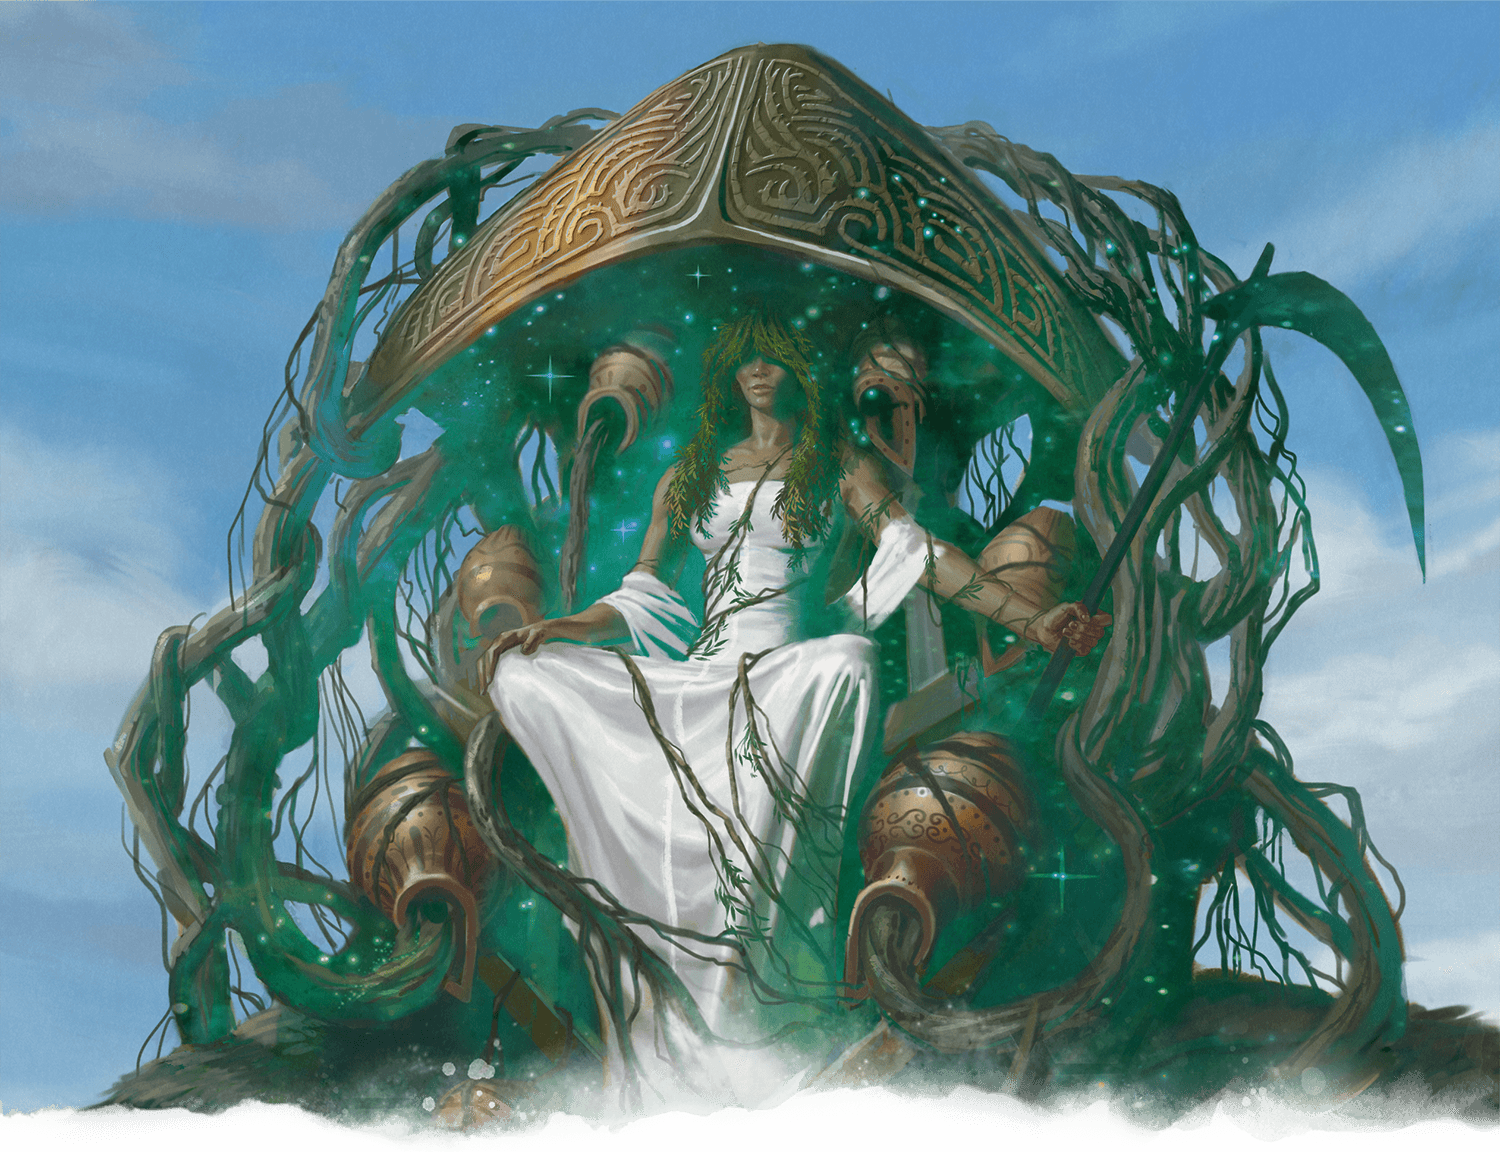
\includegraphics[width=\pdfpagewidth]{02viphoger/img/10karametra.png}};
% \end{tikzpicture}
%
% \vspace{14.5cm}

\subsection*{Keranos, God of Storms} \label{ssec::keranos}
    \subparagraph{Domains} Blue, Red.

    Keranos is the god of storms and wisdom.
    Merciless and impatient, Keranos is equally likely to strike out at mortals with a bolt of inspiration or a blast of lightning.
    To revere Keranos is to exult in the power of wisdom, clarity of purpose, and the fury of the storm.
    They are favored by tinkerers, inventors, and sailors as well as those seeking solutions to intractable problems.
    They don't tolerate the company (or the worship) of fools, and they despise vapidity and indecision.

    Keranos rarely appears directly to mortals, preferring to communicate through an epiphany or a crashing bolt of lightning.
    When they do deign to manifest in the mortal world, Keranos prefers the form of a stout, bearded, gat wearing a purple loincloth girdled in a steel chain belt with a clasp in the form of a wyvern's skull.
    Their bearing is upright and stern, with a clipped, brusque way of speaking.
    Clever plans and observations bring a hint of a smile to their face.

    % When interacting with mortals, Keranos sometimes appears in the form of a great horned owl with lightning strikes flashing in its eyes.

    % \begin{figure}[b]
    %     \centering
    %     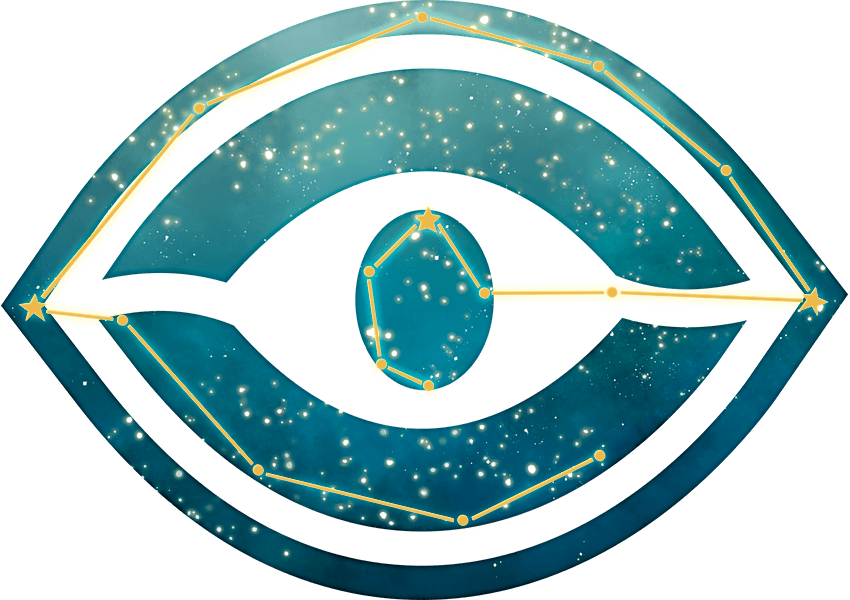
\includegraphics[width=0.47\textwidth]{02viphoger/img/10s_keranos.png}
    % \end{figure}

    \subsubsection{Worshiping Keranos}
        Keranos's name is often invoked by those amid a storm who seek safety, or by someone who is faced with a particularly difficult problem.
        Only the foolhardy call out to Keranos frivolously or in jest, since they might well smite the offender with a bolt from the blue.

        % In Akhosh, where Prince Cymede actively promoted the worship of Keranos, elaborate ceremonies are conducted beginning just before the first summer thunderstorm.
        % Intricate, open-framed sand paintings with complex geometric shapes are created by dancers in flowing blue silken wraps.
        % Then, as the rains fall, the paintings are washed away, symbolizing the impermanence of genius and the power of change.
        % Akhoash oracles strive to predict the exact time of the first storm in hopes of allowing enough time to stage the celebration.
        % A similar festival in Mephetis, called the Astrapion (``Lightning Festival''), happens during the third month of the year.
        %
        % On the last day of every month, Keranos's priests and laity bring offerings of fish and distilled spirits to their temples.
        % The fish are cooked under a skylight open to the stars, with a shot of spirits thrown on the fire.
\subsection*{Klothys, God of Destiny} \label{ssec::klothys}
    \subparagraph{Domains} Red, Gold.

    Believed to have sprung into existence during Yuadrem's earliest days, Klothys is the god of destiny and, along with Kruphix, one of the world's original deities.
    They oversee the order of the cosmos, ensuring that all things remain in their proper place, knowing how easily the cosmic balance could be undone if they were not vigilant.
    On the heels of a near-catastrophic upset of the cosmic order --- the rise to godhood and subsequent defeat of the gat Xenagos --- Klothys has emerged from Nyx for the first time in mortal memory to untangle the strands of destiny and set the world right.

    Klothys typically appears as a gat with six curling horns and an impossibly long mane of pale hair that cascades around their horns, drapes over their eyes, and spools into their spear-like weapon and the various other spindles they carry.

    Beneath their outward calm, Klothys seethes at the way mortals and gods alike have pulled apart and rearranged the threads of destiny to feed their petty ambitions.
    Their peaceful mien falls away in the presence of such villains.
    In their rage, their red-glowing eyes come into view through the veil of their hair, and they wield burning strands of hair as a devastating weapon.

    % \begin{figure}[t]
    %     \centering
    %     
\includegraphics[width=0.47\textwidth]{02viphoger/img/10s_klothys.png}
    % \end{figure}

    \subsubsection{Worshiping Klothys}
        Klothys doesn't trace their origins to mortal devotion, and they have languished in obscurity for almost the whole of Viphoger's history.
        They don't need worship to sustain or empower them, and they don't seek out reverence or demand it.
        By and large, mortals are irrelevant to them, except insofar as they have played a role in tangling the strands of destiny by defying nature's order.

\subsection*{Kruphix, God of Horizons} \label{ssec::kruphix}
    \subparagraph{Domains} Gold, Blue.

    Kruphix is the enigmatic god of mysteries, horizons, and the passage of time.
    Their followers claim that they know not only everything that is known at present, but everything that has ever been known by anyone.

    Quiet surrounds Kruphix like a shroud.
    Standing apart from the other gods, they speak rarely, even to their most favored followers.
    When they do communicate, it is often as a barely audible whisper.
    Kruphix can speak with a booming voice directly into the minds of all the other gods simultaneously, though, doing so when something threatens the cosmic order.

    Kruphix's true form is more abstract than that of any of the other gods.
    They appear only in star-filled silhouette, usually as a hooded, four-armed figure of indeterminate species and gender.
    Two of the stars in their ``body'' often shine brightly, suggesting eyes.
    Kruphix's starry silhouette sometimes takes the form of a bird or a whale.

    % \begin{figure}[b]
    %     \centering
    %     
\includegraphics[width=0.47\textwidth]{02viphoger/img/10s_kruphix.png}
    % \end{figure}

    \subsubsection{Worshiping Kruphix}
        Many pray to Kruphix when they need to find something lost, but few dedicate themselves to their worship.
        Cults devoted to Kruphix fiercely guard their secrets, and their initiates refrain from drawing attention to themselves.
        Some followers and champions of Kruphix travel the world in secret, searching for hidden truths.
        Many use secret signals to enable them to find safe lodging with other worshipers nearly anywhere.

        Rituals honoring Kruphix are usually performed at boundaries, both temporal and spatial: shorelines, riverbanks, equinoxes, and sunsets.
        One of the god's greatest festivals is the Agrypnion (``The Watching''), which marks the end of summer and the close of the year.
